\documentclass[11pt,letterpaper]{article}
\PassOptionsToPackage{hyphens}{url}
\usepackage[margin=.83in,top=.8in,bottom=.8in,headheight=15pt]{geometry}
\usepackage[T1]{fontenc}
\usepackage{lmodern,amsmath,amssymb,mathtools,bm,booktabs,array,graphicx,tikz}
\usetikzlibrary{arrows.meta,positioning,calc,decorations.pathreplacing,patterns}
\definecolor{ink}{HTML}{17344D}\definecolor{accent}{HTML}{087E8B}\definecolor{pale}{HTML}{EDF5F5}\definecolor{gold}{HTML}{AD6B19}
\providecommand{\dd}{\,\mathrm{d}}\providecommand{\R}{\mathbb{R}}
\providecommand{\E}{\mathbb{E}}\providecommand{\Var}{\operatorname{Var}}
\providecommand{\Cov}{\operatorname{Cov}}\providecommand{\diag}{\operatorname{diag}}
\providecommand{\norm}[1]{\left\lVert#1\right\rVert}
\providecommand{\abs}[1]{\left|#1\right|}
\usepackage{microtype,hyperref,fancyhdr,enumitem,amsthm,sectsty,needspace}
\allsectionsfont{\raggedright}
\hypersetup{colorlinks=true,linkcolor=ink,urlcolor=accent,pdfauthor={Zan Ahmad},pdftitle={Probability calibration and missing-modality evaluation / Lecture notes}}
\setlength{\parindent}{0pt}\setlength{\parskip}{6pt}\linespread{1.07}
\setlist{itemsep=3pt,topsep=4pt,leftmargin=*}
\emergencystretch=2em\clubpenalty=10000\widowpenalty=10000
\pagestyle{fancy}\fancyhf{}\fancyhead[L]{\small Computational Cardiology}\fancyhead[R]{\small Lecture 16}
\fancyfoot[L]{\footnotesize Zan Ahmad}\fancyfoot[R]{\footnotesize\thepage}\renewcommand{\headrulewidth}{.3pt}
\newtheorem{proposition}{Proposition}\newtheorem{theorem}{Theorem}\newtheorem{lemma}{Lemma}
\theoremstyle{definition}\newtheorem{definition}{Definition}\newtheorem{example}{Example}
\numberwithin{equation}{section}
\begin{document}
{\small\scshape Computational Cardiology\hfill Lecture 16}\par\medskip
{\raggedright\hyphenpenalty=10000\exhyphenpenalty=10000\LARGE\bfseries\color{ink} Probability calibration and missing-modality evaluation\par}\medskip
{\small Lecture notes}\par\bigskip
Ranking, classification and probability prediction are distinct mathematical properties of a score. Positive temperature scaling preserves the first two at a one-half decision threshold while changing probability values. A paired modality comparison then separates this transformation from the loss of information caused by an unavailable measurement.

\section{Group-level scores and prediction tasks}
\hypertarget{note-group-level-scores-and-prediction-tasks}{}\label{note:group-level-scores-and-prediction-tasks}
{\small \href{slides.html\#frame=three-properties-of-a-score\&step=1}{Slides for this section}}\par
A classifier can rank cases sensibly while assigning exaggerated probabilities. Discrimination asks whether higher scores tend to belong to positive outcomes. Calibration asks whether events occur at the frequency associated with the stated probabilities. A probability score evaluates the forecasts against realized outcomes. These questions overlap but are not interchangeable. In this lesson we compare a one-modality model with a two-modality model on the same unseen groups, then examine what changes when the second measurement is unavailable.

Our synthetic dataset has 360 groups with two noisy observations each and one stable binary outcome per group. Features A and B are dimensionless latent measurements, not named clinical tests. Both observations are assumed available before the prediction being evaluated. We average the two fitted logits to produce one group score, then evaluate one probability per group. This aggregation rule is fixed in advance; averaging probabilities instead would define a different model. The example makes no claim about longitudinal disease dynamics.

The group split contains 180 training groups, eighty validation groups and one hundred test groups. No group appears in two subsets. The test set contains forty-two positive outcomes in this realization. That count describes this sample rather than a disease prevalence. Keeping the evaluation cases fixed is essential when comparing extra modalities; otherwise an apparent improvement may simply reflect a different, easier subset.

For repeated observations with logits $z_{g1}$ and $z_{g2}$, this model uses
\[
 p_g=\sigma\!\left(\frac{z_{g1}+z_{g2}}2\right).
\]
In general this differs from $[\sigma(z_{g1})+\sigma(z_{g2})]/2$ because the sigmoid is nonlinear. The aggregation rule is therefore part of the predictor, not a harmless rearrangement of averages.
\section{Imputation, missingness indicators and a fixed cohort}
\hypertarget{note-imputation-missingness-indicators-and-a-fixed-cohort}{}\label{note:imputation-missingness-indicators-and-a-fixed-cohort}
{\small \href{slides.html\#frame=represent-a-missing-measurement\&step=1}{Slides for this section}}\par
The A-only model uses one standardized feature. The AB model uses A, B and a binary indicator that B was missing. Approximately one fifth of generated groups lack B in both observations. For AB, we compute the median of observed training B values, substitute that value where B is missing, and standardize the resulting three columns using training statistics. The indicator lets the model distinguish an imputed value from an actual measurement equal to the median. It does not recover the missing information.

Each logistic model is fit to the training rows with the same fixed penalty choice. Every group contributes two rows, so the training objective weights groups equally in this example. Unequal observation counts would need an explicit weighting or aggregation decision. Validation and test transformations use the stored median, mean and scale; they never recompute them. The code rejects a training AB dataset with no observed B values because that dataset cannot teach the intended B relationship.

The comparison retains test cases with missing B. Dropping them would change the population and conceal the behavior of the actual missing-data rule. Likewise, a complete-case AB score should not be compared with an A score over all cases without showing the subset difference. The fitted preprocessing and the eligible-case definition are part of the predictive method, not administrative details.

With training median $m_B$, represent a missing second modality by $B^*=m_B$ together with $r_B=1$; observed values use $B^*=B$ and $r_B=0$. The indicator lets a linear logit distinguish an imputation from an actual observation equal to the median. It cannot reconstruct the unmeasured value. Both imputation and standardization remain frozen when evaluating missing-modality cases.
\section{Positive temperature scaling}
\hypertarget{note-positive-temperature-scaling}{}\label{note:positive-temperature-scaling}
{\small \href{slides.html\#frame=temperature-scaled-probabilities\&step=1}{Slides for this section}}\par
To create a visible calibration exercise, we deliberately multiply each fitted group logit by 2.5. This makes scores more extreme without changing their ordering or their side of zero. We label these as sharpened scores throughout. It is a controlled intervention, not evidence that every logistic model is intrinsically overconfident. A positive temperature divides the sharpened logit before the sigmoid. Temperatures above one soften the scores toward one half; temperature one leaves them unchanged.

Guo and colleagues describe temperature scaling as a single positive parameter selected using validation likelihood. Our binary adaptation searches temperatures between 0.2 and 5 by minimizing mean validation cross-entropy over eighty groups. The base model and preprocessing remain fixed. The test labels do not choose the temperature. The fitted values are about 1.864 for A and 1.670 for AB in this realization. A zero logit vector cannot identify temperature, so the implementation rejects that degenerate calibration input.

For finite positive temperature, dividing logits preserves their order and signs. Because the sigmoid is increasing, ranking and decisions at probability threshold 0.5 remain unchanged. This is a mathematical property of this transformation, not a promise that every calibration method preserves ranking. Decisions at some other fixed threshold can change. Nor does successful validation fitting guarantee improved calibration on every future population.

\[
p_T=\sigma(z/T),\qquad T>0
\]
z already includes the declared 2.5 teaching multiplier. T is fitted on validation groups only; it is dimensionless.

For $T>0$, $z_i>z_j$ implies $z_i/T>z_j/T$, and $\sigma$ is strictly increasing. Thus pairwise rankings and ties are unchanged. Also
\[
 \sigma(z/T)\ge\tfrac12\quad\Longleftrightarrow\quad z\ge0.
\]
At another threshold $p_*$, the equivalent logit condition is $z\ge T\log[p_* /(1-p_*)]$, which can change with $T$.
\section{Proper probability scores and reliability bins}
\hypertarget{note-proper-probability-scores-and-reliability-bins}{}\label{note:proper-probability-scores-and-reliability-bins}
{\small \href{slides.html\#frame=the-brier-score-panel-1\&step=1}{Slides for this section}}\par
The Brier score averages squared differences between predicted probabilities and binary outcomes. A forecast of one for an outcome of zero contributes one; a forecast of one half contributes one quarter regardless of the label. Its minimum is zero for perfect forecasts. A lower score is useful evidence about probability prediction, but it can reflect improved discrimination as well as calibration. The scikit-learn calibration documentation explicitly cautions against interpreting Brier score as calibration alone.

Our reliability plot uses five fixed probability intervals. Each point shows the mean probability and observed event fraction among the test groups in that interval. Empty bins are omitted, and their zero counts remain in the results file. A point based on a handful of groups is noisier than one based on many groups. Read those counts before interpreting deviations from the diagonal. A line connecting the bin summaries does not establish calibration between them, and a small test sample cannot establish exact calibration everywhere.

For AB, temperature scaling changes test Brier score from about 0.2306 to 0.2083, while AUC stays about 0.7455 and accuracy at threshold 0.5 stays 0.67. The unchanged ranking follows the transformation; the improved score is an empirical result for these groups. AUC is computed by comparing every positive-negative score pair, awarding half credit for ties. If either true class is absent, this comparison is unavailable rather than automatically excellent.

\[
\mathrm{Brier}=\frac1N\sum_{i=1}^{N}(p_i-y_i)^2
\]
N is the number of evaluated groups; probabilities and binary labels are dimensionless. This is the binary, unscaled convention.

If $Y\mid X$ is Bernoulli with true event probability $\eta$, then
\[
 \mathbb E[(p-Y)^2\mid X]=(p-\eta)^2+\eta(1-\eta).
\]
The first term is minimized at $p=\eta$; the second is irreducible outcome variability. This explains the probability interpretation of the Brier score, without making a finite-sample Brier change a pure measure of calibration. For ranking,
\[
 \mathrm{AUC}=\frac1{N_+N_-}\sum_{i:y_i=1}\sum_{j:y_j=0}
 [\boldsymbol1_{p_i>p_j}+\tfrac12\boldsymbol1_{p_i=p_j}].
\]
\begin{center}\begin{minipage}{.98\linewidth}\centering
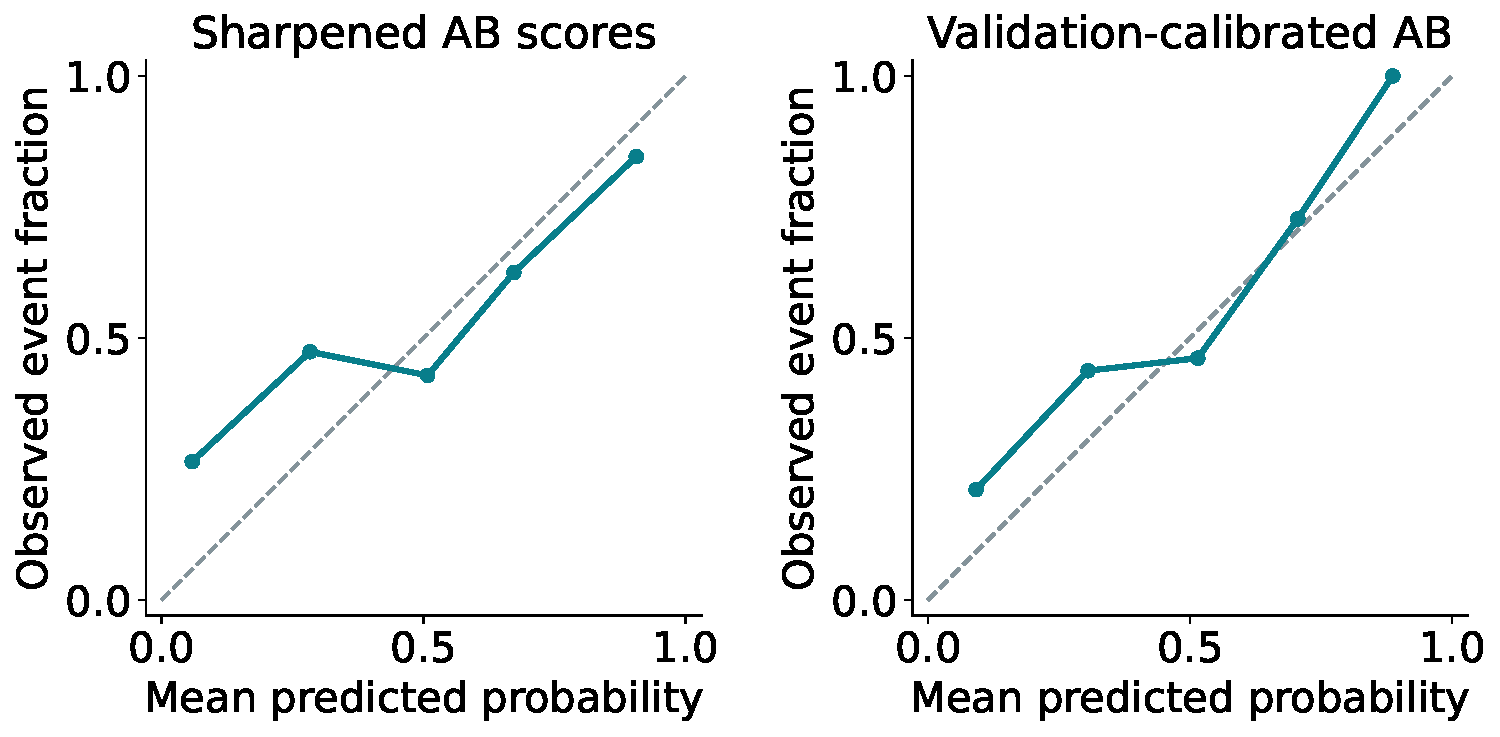
\includegraphics[width=.96\linewidth,height=.57\textheight,keepaspectratio]{calibration.pdf}\par\smallskip
{\small AB reliability diagrams on the same 100 test groups, before and after validation-fitted temperature scaling. The raw group logits were deliberately sharpened by 2.5. Five fixed bins are used; their counts are in results.json.}
\end{minipage}\end{center}
\section{A paired missing-modality intervention}
\hypertarget{note-a-paired-missing-modality-intervention}{}\label{note:a-paired-missing-modality-intervention}
{\small \href{slides.html\#frame=the-paired-modality-comparison\&step=1}{Slides for this section}}\par
After calibration, the A-only model has test Brier score about 0.2352, compared with 0.2083 for AB. The comparison includes the same one hundred groups. To probe reliance on B, we remove additional B observations from nested sets of test groups using a separate fixed random seed. Nineteen groups originally lack B; the intermediate and final scenarios have sixty-one and one hundred groups without it. The imputation rule, feature scales, fitted coefficients and temperatures stay frozen.

The AB Brier score rises to about 0.2206 and then 0.2363 as B disappears. The A-only score stays unchanged because that model does not use B. Complete B removal does not force AB to equal A: its A coefficient, intercept, missingness-indicator coefficient and temperature were learned in a different model. A result near the A baseline in this run is therefore an observed comparison, not an algebraic identity.

This stress test answers a specific intervention question. Missingness in practice may depend on illness, access, workflow or prior decisions, whereas our additional removal is random across fixed test groups. We have not measured performance under every such process. Report the missingness pattern and retain all affected cases; do not convert a successful toy stress test into a claim of universal robustness.

Paired evaluation holds the group identifiers and outcomes fixed, then replaces the extra measurement by the model's prescribed missing-data representation. The resulting difference measures sensitivity to that information loss under this intervention. It does not isolate a causal biological effect of the modality, and it does not establish robustness to every missingness mechanism.
\begin{center}\begin{minipage}{.98\linewidth}\centering
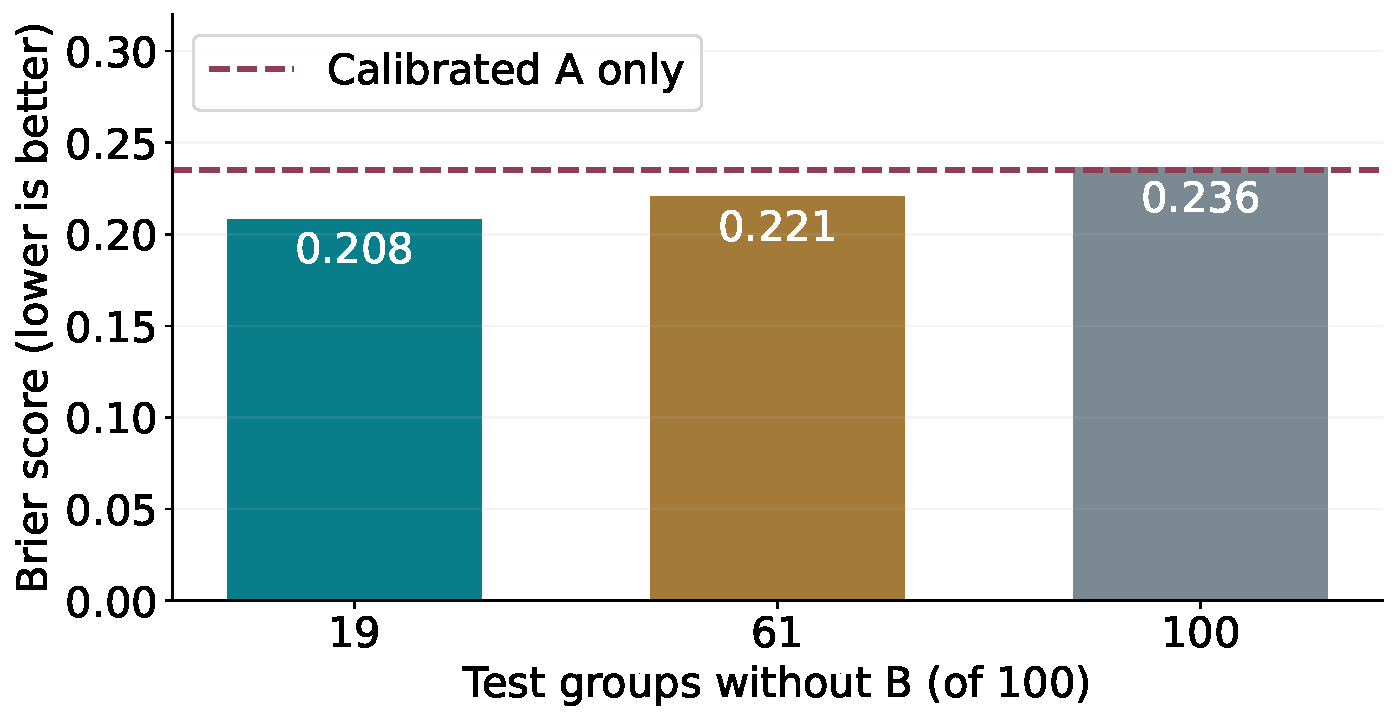
\includegraphics[width=.96\linewidth,height=.57\textheight,keepaspectratio]{missing-modality.pdf}\par\smallskip
{\small Frozen calibrated AB model on identical test groups with 19, 61 and 100 groups lacking B. Brier score rises from 0.2083 to 0.2206 to 0.2363. The unchanged A-only baseline is 0.2352.}
\end{minipage}\end{center}
\section{Calibration and distribution dependence}
\hypertarget{note-calibration-and-distribution-dependence}{}\label{note:calibration-and-distribution-dependence}
{\small \href{slides.html\#frame=distribution-dependent-calibration\&step=1}{Slides for this section}}\par


Calibration is distribution dependent. If $P(Y=1\mid z)$ changes between validation and a future population, the same fitted temperature need not produce calibrated probabilities. A reliability bin estimates one conditional event fraction using a finite count; empty bins supply no estimate. The model and temperature are fixed before test evaluation, but uncertainty in that evaluation remains.
\bigskip
\section*{Exercises}
\par\noindent\begin{minipage}{\linewidth}
\subsection*{AC16-E1. Separate rank from probability error}
Four outcomes are [0,1,0,1]. Model P predicts [0.2,0.4,0.6,0.8]; model Q predicts [0.1,0.3,0.7,0.9].

\textbf{a} Compute the Brier score of each model.

\end{minipage}\par\medskip
\textbf{b} Compute the pairwise AUC for each.

\textbf{c} What does this comparison establish, and what does it not establish about calibration?

\par\noindent\begin{minipage}{\linewidth}
\subsection*{AC16-E2. Trace a temperature transform}
A sharpened logit is log(4), so its original probability is 0.8. Apply temperature T=\allowbreak{}2.

\textbf{a} Find the new probability exactly.

\end{minipage}\par\medskip
\textbf{b} Does the predicted class change at thresholds 0.5 and 0.7?

\textbf{c} Which split chooses T, and why is an all-zero logit vector uninformative for this choice?

\par\noindent\begin{minipage}{\linewidth}
\subsection*{AC16-E3. Audit a modality comparison}
A two-modality model is evaluated only on 60 complete cases and has Brier 0.18. A one-modality model is evaluated on all 100 cases and has Brier 0.22.

\textbf{a} Can these numbers alone establish that the extra modality improves the same target population?

\end{minipage}\par\medskip
\textbf{b} Give a comparison that isolates the model difference, and state a limitation if only complete cases are used.

\textbf{c} For an all-case evaluation with missing B, name three fitted quantities that must remain frozen during test evaluation.

\par\noindent\begin{minipage}{\linewidth}
\subsection*{AC16-E4. Assignment 4 evaluation report}
Use the supplied experiment to produce a concise, reproducible comparison. Feedback points do not add a new course weight.

\textbf{a} Specify the split, group aggregation and missing-data preprocessing.

\end{minipage}\par\medskip
\textbf{b} Report the declared confidence intervention, calibration choice and paired test comparison.

\textbf{c} Describe the frozen missingness stress test and its result.

\textbf{d} Identify one reliability-bin issue and one generalization limitation.

\section*{References}
\noindent\begin{minipage}{\linewidth}
Zan Ahmad, Advanced Topics in Computational Cardiology syllabus, Fall 2024. PDF pages 1--2.

\end{minipage}\par\medskip
\noindent\begin{minipage}{\linewidth}
scikit-learn, Probability calibration. Sections 1.16.1, 1.16.2 and 1.16.3.4; introductory note on proper scoring rules.

\url{https://scikit-learn.org/stable/modules/calibration.html}
\end{minipage}\par\medskip
\noindent\begin{minipage}{\linewidth}
Guo, Pleiss, Sun and Weinberger, On Calibration of Modern Neural Networks (2017). PDF page 4, Section 4 introduction; PDF page 6, Section 4.2 temperature-scaling paragraph and equation (9).

\url{https://proceedings.mlr.press/v70/guo17a.html}
\end{minipage}\par\medskip
\noindent\begin{minipage}{\linewidth}
scikit-learn, Common pitfalls and recommended practices. Sections 12.1, 12.2 and 12.2.1.

\url{https://scikit-learn.org/stable/common_pitfalls.html}
\end{minipage}\par\medskip
\end{document}
